Access to parking places is a  challenge in many urban areas such as universities, shopping malls, hospitals, where there is a high demand for parking spaces and a limited number of them in availability\cite{parmar_study_2020}.\\\\
Makerere University in collaboration with KSA in 2014 put in a place an automated parking system that allows motorists to purchase tickets and make payments at any of the payment points within the university premises to ensure the smooth flow of traffic, reducing congestion, and generating revenue for the university\cite{wamai_mak_2014}.\\\\ The current system of ticketing and payment for parking at Makerere University in Kampala, Uganda, has however suffered from several problems, such as frequent malfunction of the ticketing machines, fraud by the system employees who may sometimes take payments from motorists direct rather than having motorists pay at the paypoints within the university, difficulty in locating a payment point for motorists, and hefty fines for lost tickets. These problems result in inconvenience, inefficiency, and revenue loss for both the system’s managers and motorists.

To address these problems, we propose a novel system in the local context that consists of a mobile app that enables cashless digital prepayment of the parking fees using local popular payment platforms such as MTN mobile money, Airtel Money. A study found that in Sub-Saharan Africa, the use of mobile money platforms has neem of great impact, promoting financial inclusion, with 548 million registered mobile money accounts in the region. These platforms have seen a 23\% growth in transaction value, reaching 490 billion dollars\cite{centellegher_mobile_2018}. Another study found that in Uganda, mobile money accounts are held by 43\% of the population, compared to just 11\% who have bank accounts\cite{baah_state_2021}.This demonstrates how widely used these platforms are in the region.


Our work is also motivated by a growing trend of using mobile apps for parking payment in some cities around the world. Mobile applications offer several advantages over traditional methods of parking payment, such as convenience, flexibility, security, and cost-effectiveness, amongst others. A report by Grand View Research also indicates that the global mobile parking app market size was valued at USD 6.4 billion in 2020 and is expected to grow at a compound annual growth rate (CAGR) of 22.1\% from 2021 to 2028\cite{GrandViewResearch2023}. Some examples of mobile parking applications include ParkMobile \cite{ParkMobile2023} developed and used in the United States and Flowbird developed in France\cite{Flowbird2023}. Most of these applications are designed for developed countries with advanced infrastructure and technology. There is a need for developing context-specific solutions that cater to the needs as well as limited resources in developing countries like Uganda.


\begin{figure}[h]
    \begin{center}
        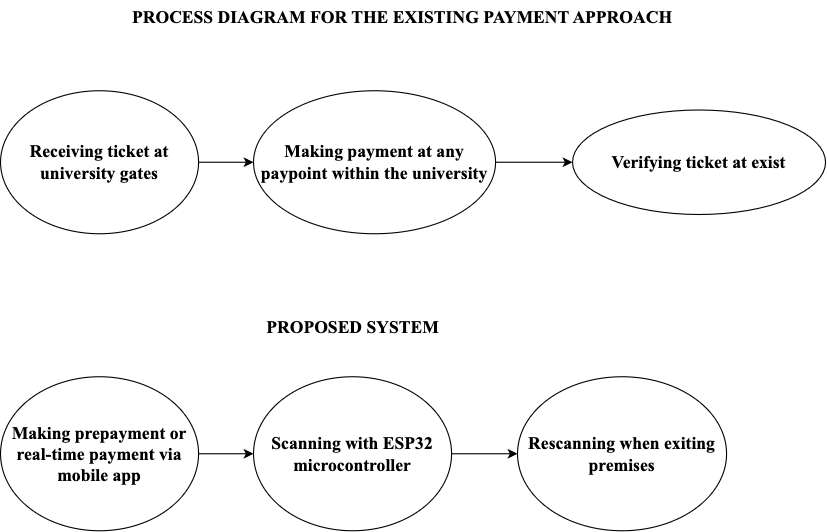
\includegraphics[scale = 0.4]{images/process}
        \caption{High level Process diagram comparing the existing and proposed system}
    \end{center}
\end{figure}


\clearpage